%%%%%%%%%%%%%%%%%%%%%%%%%%%%%%%%%%%%%%%%%%%%%%%%%%%%%%%%%%%%%%%%%%%%%%%%%%%%%%%%%%%%%%%%%%%%%%%%%%%%%
% This template is distributed with ABSOLUTELY NO WARRANTY.
% It serves as a guideline and constitutes a basic structure for a
% thesis/dissertation. The user assumes full responsibility for formatting
% and typesetting their document and for verifying that all the thesis
% requirements set by the University of Tennessee are met. Please refer to the most
% recent UT thesis guide (http://web.utk.edu/~thesis/thesisresources.shtml)
% or contact the thesis consultant (http://web.utk.edu/~thesis/).
% Please report any bugs to the thesis consultant.
%%%%%%%%%%%%%%%%%%%%%%%%%%%%%%%%%%%%%%%%%%%%%%%%%%%%%%%%%%%%%%%%%%%%%%%%%%%%%%%%%%%%%%%%%%%%%%%%%%%%%
% O P T I O N S:
% 1. thesis/dissertation
% 2. monochrome
% 3. all options provided by the report class
\documentclass[thesis,letterpaper,12pt]{utthesis} % thesis, one side
% some alternatives are:
%\documentclass[thesis,monochrome,letterpaper,12pt]{utthesis} %thesis, one side, monochrome text
%\documentclass[thesis,twoside,letterpaper,12pt]{utthesis} % thesis, two side
%\documentclass[thesis,monochrome,twoside,letterpaper,12pt]{utthesis} % thesis, two side, monochrome text
% for a dissertation, replace the thesis option by dissertation:
% \documentclass[dissertation,letterpaper,12pt]{utthesis} . . .
\renewcommand{\baselinestretch}{1.5} 	 % line Spacing
%%%%%%%%%%%%%%%%%%%%%%%%%%%%%%%%%%%%%%%%%%%%%%%%%%%%%%%%%%%%%%%%%%%%%%%%%%%%%%%%%%%%%%%%%%%%%%%%%%%%%
% TO DO: FILL IN YOUR INFORMATION BELOW - READ THIS SECTION CAREFULLY
%%%%%%%%%%%%%%%%%%%%%%%%%%%%%%%%%%%%%%%%%%%%%%%%%%%%%%%%%%%%%%%%%%%%%%%%%%%%%%%%%%%%%%%%%%%%%%%%%%%%%
\title{My Thesis or Dissertation Title}	       % title of thesis/dissertation
\author{My Name}                % author's name
\copyrightYear{2012}            % copyright year of your thesis/dissertation
\graduationMonth{May}           % month of graduation of your thesis/dissertation
\majorProfessor{My Advisor}	    % advisor's name
\keywords{List, Of, Keywords}	% keywords (optional) separated by commas - these are used in the PDF file properties
\viceProvost{Carolyn R. Hodges} % vice provost name
\major{Mechanical Engineering}	% major: Mechanical Engineering, Aerospace Engineering, Mathematics...
\degree{Master of Science}	    % degree: Doctor of Philosophy, Master of Science, Master of Engineering...
\college{Engineering}           % college
\dept{Mechanical, Aerospace and Biomedical Engineering}	% department
\university{The University  of Tennessee, Knoxville}	% school name
% THIS TEMPLATE ACCOMMODATES UP TO 5 COMMITTEE MEMBERS - ENTER ONLY THE NAMES OF THE MEMBERS ON YOUR COMMITTEE
\numberOfCommitteeMembers{2} % enter the number of committee members
\committeeMemberA {Committee Member 1}	% name of first committee member
\committeeMemberB {Committee Member 2}	% name of second committee member
\committeeMemberC {Committee Member 3}	% ... you get the trend!
\committeeMemberD {Committee Member 4}	% if your committee has less than 4 members, you do not need to edit the
\committeeMemberE {Committee Member 5}  % rest of committee names
%%%%%%%%%%%%%%%%%%%%%%%%%%%%%%%%%%%%%%%%%%%%%%%%%%%%%%%%%%%%%%%%%%%%%%%%%%%%%%%%%%%%%%%%%%%%%%%%%%%%%
% LOAD SOME USEFUL PACKAGES
%%%%%%%%%%%%%%%%%%%%%%%%%%%%%%%%%%%%%%%%%%%%%%%%%%%%%%%%%%%%%%%%%%%%%%%%%%%%%%%%%%%%%%%%%%%%%%%%%%%%%
\usepackage{nomencl}                    % produces a nomenclature
\usepackage{float}                      % figure floats
\usepackage{natbib}                     % this package allows you to link your references
\usepackage{graphicx}					% graphics package
\graphicspath{ {figures/}{figures/eps/}{figures/pdf/} }% specify the path where figures are located
\usepackage{fancyhdr}                   % fancy headers and footers
\usepackage{url}                        % nicely format url breaks
\usepackage[inactive]{srcltx}		 	% necessary to use forward and inverse searching in DVI
\usepackage{relsize}                    % font sizing hierarchy
\usepackage{booktabs}                   % professional looking tables
\usepackage[config, labelfont={bf}]{caption,subfig} % nice sub figures
\usepackage{mathrsfs}                   % additional math scripts
%%% PACKAGES THAT ARE PRELOADED WITH THE CLASS ARE: amsmath,amsthm,amssymb,setspace,geometry,hyperref,and color
%%%%%%%%%%%%%%%%%%%%%%%%%%%%%%%%%%%%%%%%%%%%%%%%%%%%%%%%%%%%%%%%%%%%%%%%%%%%%%%%%%%%%%%%%%%%%%%%%%%%%
\begin{document}
    \pagenumbering{alph} % this is needed to clear certain issues with the hyperref package
    %
    \makeApprovalPage % make the approval page - this is the page that needs to be signed & returned to the thesis/dissertation consultant
    \makeETDApprovalPage % make the Electronic Thesis & Dissertation page - this page is kept with the electronic copy
    %
    \addToPDFBookmarks{0}{Front Matter}{rootNode} % create a root node named "Front Matter" in the pdf bookmarks
    \addToPDFBookmarks{1}{Title}{a} % add a pdf bookmark to the title page
    \makeTitlePage % make the title page. Make sure you properly set the \docType
    %
    \pagenumbering{roman}
    \setcounter{page}{2}
    %
    \makeCopyrightPage % make the copyright page
    %
    \addToPDFBookmarks{1}{Dedication}{b} % add a pdf bookmark to the dedication page
    \chapter*{}
\begin{center}
{\centering \it To my parents,
Mark and Sandra Bohling,
for their love and support in all my endeavours}
\end{center}  % include the dedication
    %
    \addToPDFBookmarks{1}{Acknowledgements}{c} % add a pdf bookmark to the acknowledgements page
    \chapter*{Acknowledgements}
I would like to thank the Materials Properties Council under the direction of Dr. Martin Prager and the Center for Materials Processing, directed by Dr. Claudia Rawn through the Department of Materials Science and Engineering at the University of Tennessee, Knoxville, for providing funding support for my work.  % include the acknowledgements
    %
    \addToPDFBookmarks{1}{Quote}{d} % add a pdf bookmark to the quotation page
    \chapter*{}
{\it Some quotation...} % include a quote
    %
    \addToPDFBookmarks{1}{Abstract}{e} % add a pdf bookmark to the abstract page
    \chapter*{Abstract}\label{ch:abstract}
Steam reforming of hydrocarbons is an important process for the production of hydrogen for industrial needs, such as ammonia synthesis. Due to the high temperature (\SIrange[range-phrase=--]{700}{900}{\degreeCelsius}) conditions, reformer furnace components require materials with excellent creep properties and thus highly alloyed austenitic stainless steels are typically employed. For reformer outlet manifolds, a cast, heat-resistant stainless steel with the composition 20Cr-32Ni-1Nb (ASTM A351 Grade CT15C) is widely used. However, after service exposure this alloy exhibits problems with liquation cracking in the base metal \gls{haz} during repair welding. In the work presented herein, two heats of material from centrifugally-cast manifold components were evaluated to quantify the potential susceptibility to \gls{haz} liquation cracking. The weldability of the 20Cr-32Ni-1Nb materials was evaluated using the Gleeble\texttrademark{} hot ductility test to determine the on-heating and on-cooling ductility (percent reduction in area) at various temperatures after exposure to a simulated welding thermal cycle. The as-received materials and selected hot ductility samples were characterized using \gls{olm} and \gls{sem} with \gls{eds} to correlate the hot ductility behavior with microstructural characteristics.

Both 20Cr-32Ni-1Nb heats showed similar hot ductility behavior when tested (\emph{i}) on-heating and (\emph{ii}) on-cooling from the measured \gls{zdt} of \SmartUnit{fahrenheit=2375}. The hot ductility curves revealed that both materials exhibited a poor recovery of on-cooling ductility (Class C3 based on the Nippes criteria) after exposure to the \gls{zdt}, with a noticeable \gls{zdr} and a low \gls{drr} on the order of 20\%. The microstructural evaluation revealed that the loss of on-heating and on-cooling ductility was a result of liquation along the interdendritic boundaries. \gls{eds} analysis did not reveal the presence of significant amounts of Ni-Nb-Si enriched phases adjacent to the niobium carbides. The observed liquation along the interdendritic boundaries was attributed to constitutional liquation of niobium carbides which were present in the boundary regions. Based on these findings, the two 20Cr-32Ni-1Nb heats are sensitive to \gls{haz} liquation cracking when exposed to a thermal cycle as would be encountered in repair welding.




%Repair welding of heat-resistant stainless steels used in steam reformer furnace components can be problematic if the material is in the service-exposed condition, due to liquation cracking in the base metal heat-affected zone (HAZ).  Service-exposed, cast 20Cr-32Ni-1Nb heat-resistant steel extracted from a reformer outlet manifold was evaluated using the Gleeble hot ductility test to determine its susceptibility to HAZ liquation cracking.  The hot ductility curves revealed that the service-exposed material exhibited poor ductility recovery when tested upon cooling from the on-heating zero ductility temperature (ZDT) of 2375°F.  On this basis, the service-exposed 20Cr-32Ni-1Nb material would be classified as fairly susceptible to HAZ liquation cracking when exposed to a welding thermal cycle. % your abstract
    %
    \addToPDFBookmarks{0}{Table of Contents}{f}
    \tableofcontents % generate a table of contents
    %
    \addToTOC{List of Tables} % this will add the list of tables to the Table of Contents (TOC)
    \listoftables % generate a list of tables
    %
    \addToTOC{List of Figures} % this will add the list of figures to the Table of Contents (TOC)
    \listoffigures % generate a list of figures
    %
    \makenomenclature % OPTIONAL
    \addToPDFBookmarks{0}{Nomenclature}{g} % OPTIONAL
    \printnomenclature[1.25in] % OPTIONAL
    %
    \newpage
    \pagenumbering{arabic}
    \setcounter{page}{1}
    %%%%%%%%%%%%%%%%%%%%%%%%%%%%%%%%%%%%%%%%%%%%%%%%%%%%%%%%%%%%%%%%%%%%%%%%%%%%%%%%%%%%%%%%%%%%%%%%%%%%%
    % INCLUDE THE CHAPTERS STARTING WITH THE NOMENCLATURE IF PRESENT
    %%%%%%%%%%%%%%%%%%%%%%%%%%%%%%%%%%%%%%%%%%%%%%%%%%%%%%%%%%%%%%%%%%%%%%%%%%%%%%%%%%%%%%%%%%%%%%%%%%%%%
    %!TEX root = ..\ms-thesis.tex
% enter the list of nomenclature here
\nomenclature{HAZ}{Heat-affected zone}
 % OPTIONAL
    %!TEX root = ..\ms-thesis.tex
\chapter{Introduction} \label{ch:introduction}

Steam reforming of hydrocarbons is an important industrial process for the production of hydrogen gas either as an end product or as an input for other processes such as ammonia synthesis and petroleum hydrocracking. In the steam reforming process, a hydrocarbon feedstock is reacted with steam, usually in the presence of a catalyst, to yield hydrogen gas and byproducts according to the following reactions \cite{rostrup-nielsen_catalytic_1984}:
\begin{align}
%\ce{C_{n}H_{m}}+\ce{n H2O} -> \ce{n CO}+\bigl(n+\frac{m}{2}\bigr)\ce {H2} \quad (-\Delta{}H^{0}_{298} < 0) \\
\ce{C_{n}H_{m} + n H2O -> n CO + } \bigl(n + \frac{m}{2}\bigr) \ce{H2} \quad (-\Delta{}H^{0}_{298} < 0) \label{eq:1} \\
\ce{CO + H2O <=> CO2 + H2} \quad (-\Delta{}H^{0}_{298} = 41.2 \, \text{kJ mol}^{-1}) \label{eq:2} \\
\ce{CO + 3H2 <=> CH4 + H2O} \quad (-\Delta{}H^{0}_{298} = 206.2 \, \text{kJ mol}^{-1}) \label{eq:3}
\end{align}
Most commonly, methane (CH$_{\textnormal{4}}$) in the form of natural gas is the preferred feedstock, although heavier hydrocarbons such as propane, naphtha, and heptane can be used depending upon availability and cost \cite{rostrup-nielsen_catalytic_1984,haussinger_hydrogen_2000}. In the above reactions, steam functions as an oxiziding agent to break apart the hydrocarbon; in some variants of the process, air is also added as a further oxidizer. The catalyst is typically nickel-based on an oxide substrate.

By adjusting the process conditions (exit temperature and amount of steam), the equilibria of the reforming reactions \ref{eq:1}--\ref{eq:3} can be modified to favor certain products and thereby adjust the composition of the product gas. For example, for ammonia synthesis which is one of the largest industrial consumers of hydrogen, the typical desired process conditions are 3.3 MPa exit pressure, 800C exit temperature, and a steam to carbon ratio of 3.7 \cite{rostrup-nielsen_catalytic_1984} to minimize the methane content in the product. Considering that reaction \ref{eq:1} is endothermic while reactions \ref{eq:2} and \ref{eq:3} are exothermic, under the process conditions just listed (for minimizing methane) the overall reaction is endothermic and thus external heating is required. The necessary heat is supplied by enclosing the reaction apparatus in a \emph{reformer furnace}.

An illustration of a typical reformer furnace is shown in Figure~\ref{fig:reformer-furnace}. The furnace is a tubular reformer design, in which the feedstock stream (e.g. containing natural gas and steam) is fed simultaneously through a series of identical tubes, containing the catalyst material, which are externally heated. These tubes are visible in Figure~\ref{fig:reformer-furnace} in a vertical arrangement, with the burners installed on the sides of the furnace walls. The inlet side where the preheated feedstock enters the tubes is at the top of the furnace, with the hot product gas mixture collected at an outlet manifold at the bottom of the furnace, consisting of ``hot side'' header, tee, and reducer ("cone") which connects to a refractory-walled transfer line. Through the transfer line, the product gas flow is directed to a waste heat recovery boiler which generates high-pressure steam to be used in the reformer \cite{rostrup-nielsen_catalytic_1984}. A photograph of another furnace is shown in Figure~\ref{fig:reformer-tee-cone} \cite{penso_repair_2006} in which the outlet pigtails (from the reformer tubes), the outlet header and tee, and cone are clearly visible.

\begin{figure}[h]
\centering
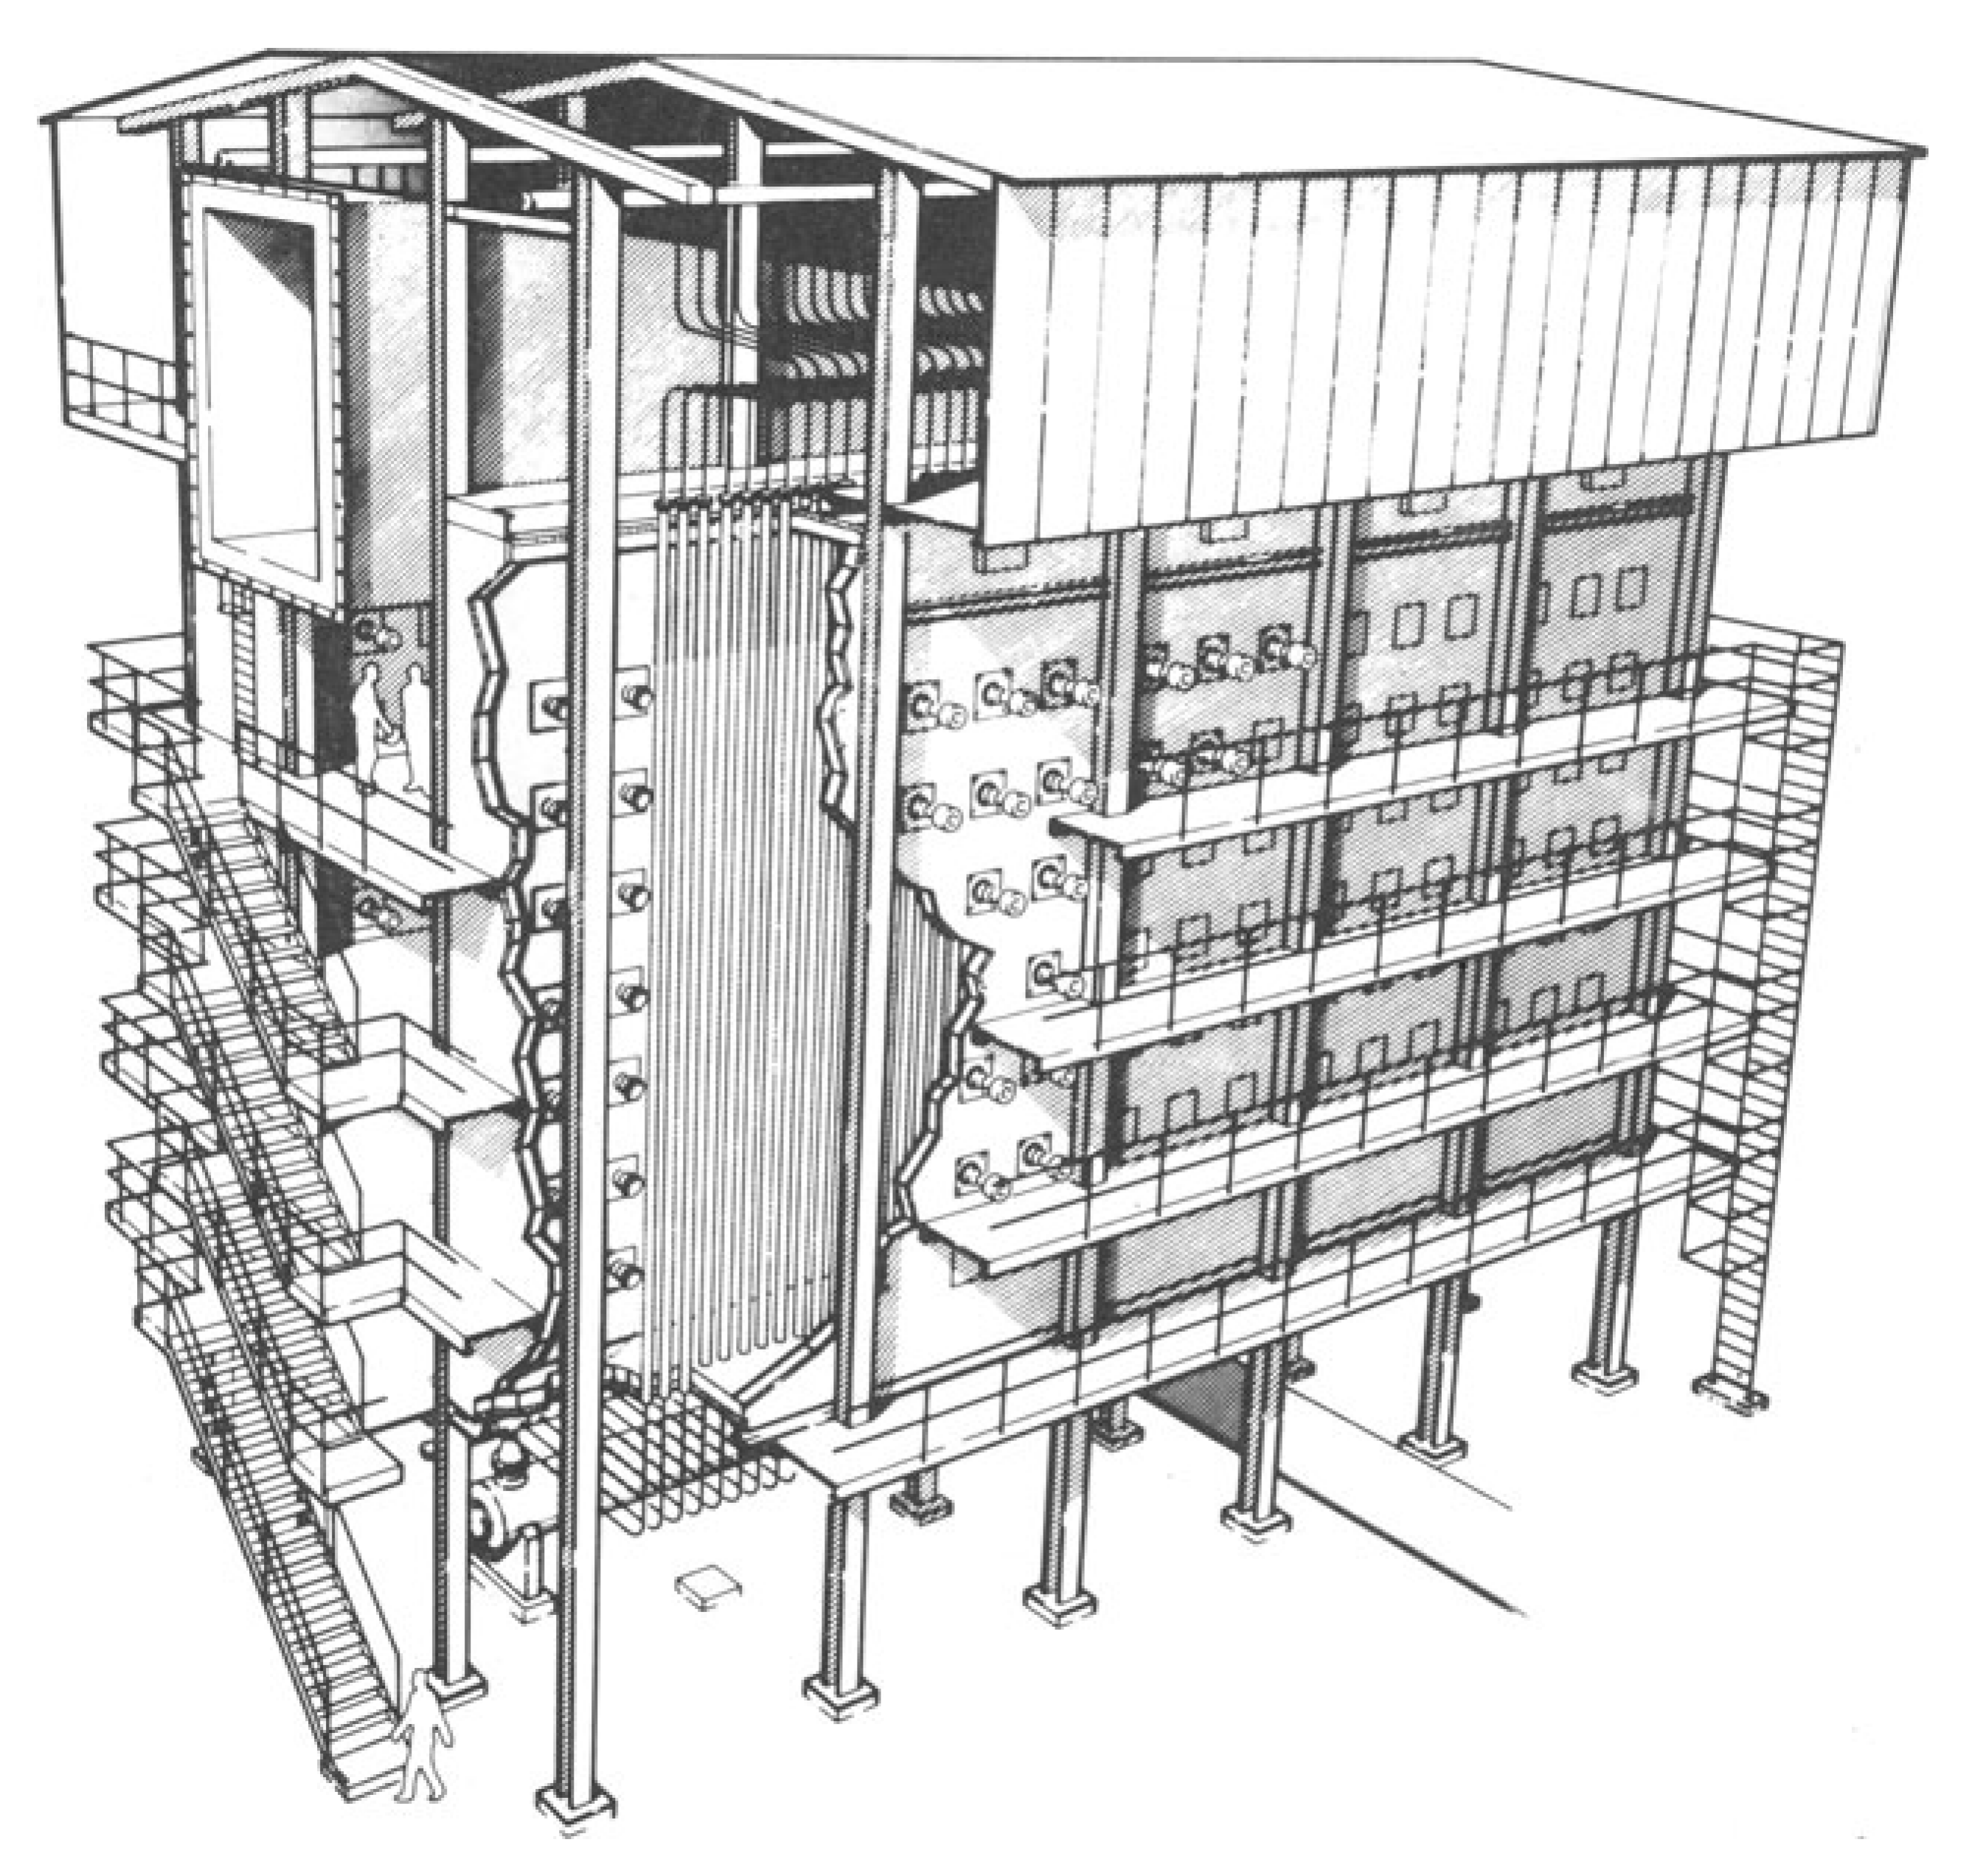
\includegraphics{figures/reformer-furnace}
\caption{Illustration of a typical reformer furnace. The reformer catalyst tubes are arranged vertically, with side-mounted burners on both walls. The pre-heated feedstock gas mixture enters the tubes from the top and the product gas is collected in an outlet manifold at the bottom of the furnace.  From \citet[Fig.~9]{rostrup-nielsen_catalytic_1984}.}
\label{fig:reformer-furnace}
\end{figure}

\begin{figure}[h]
\centering
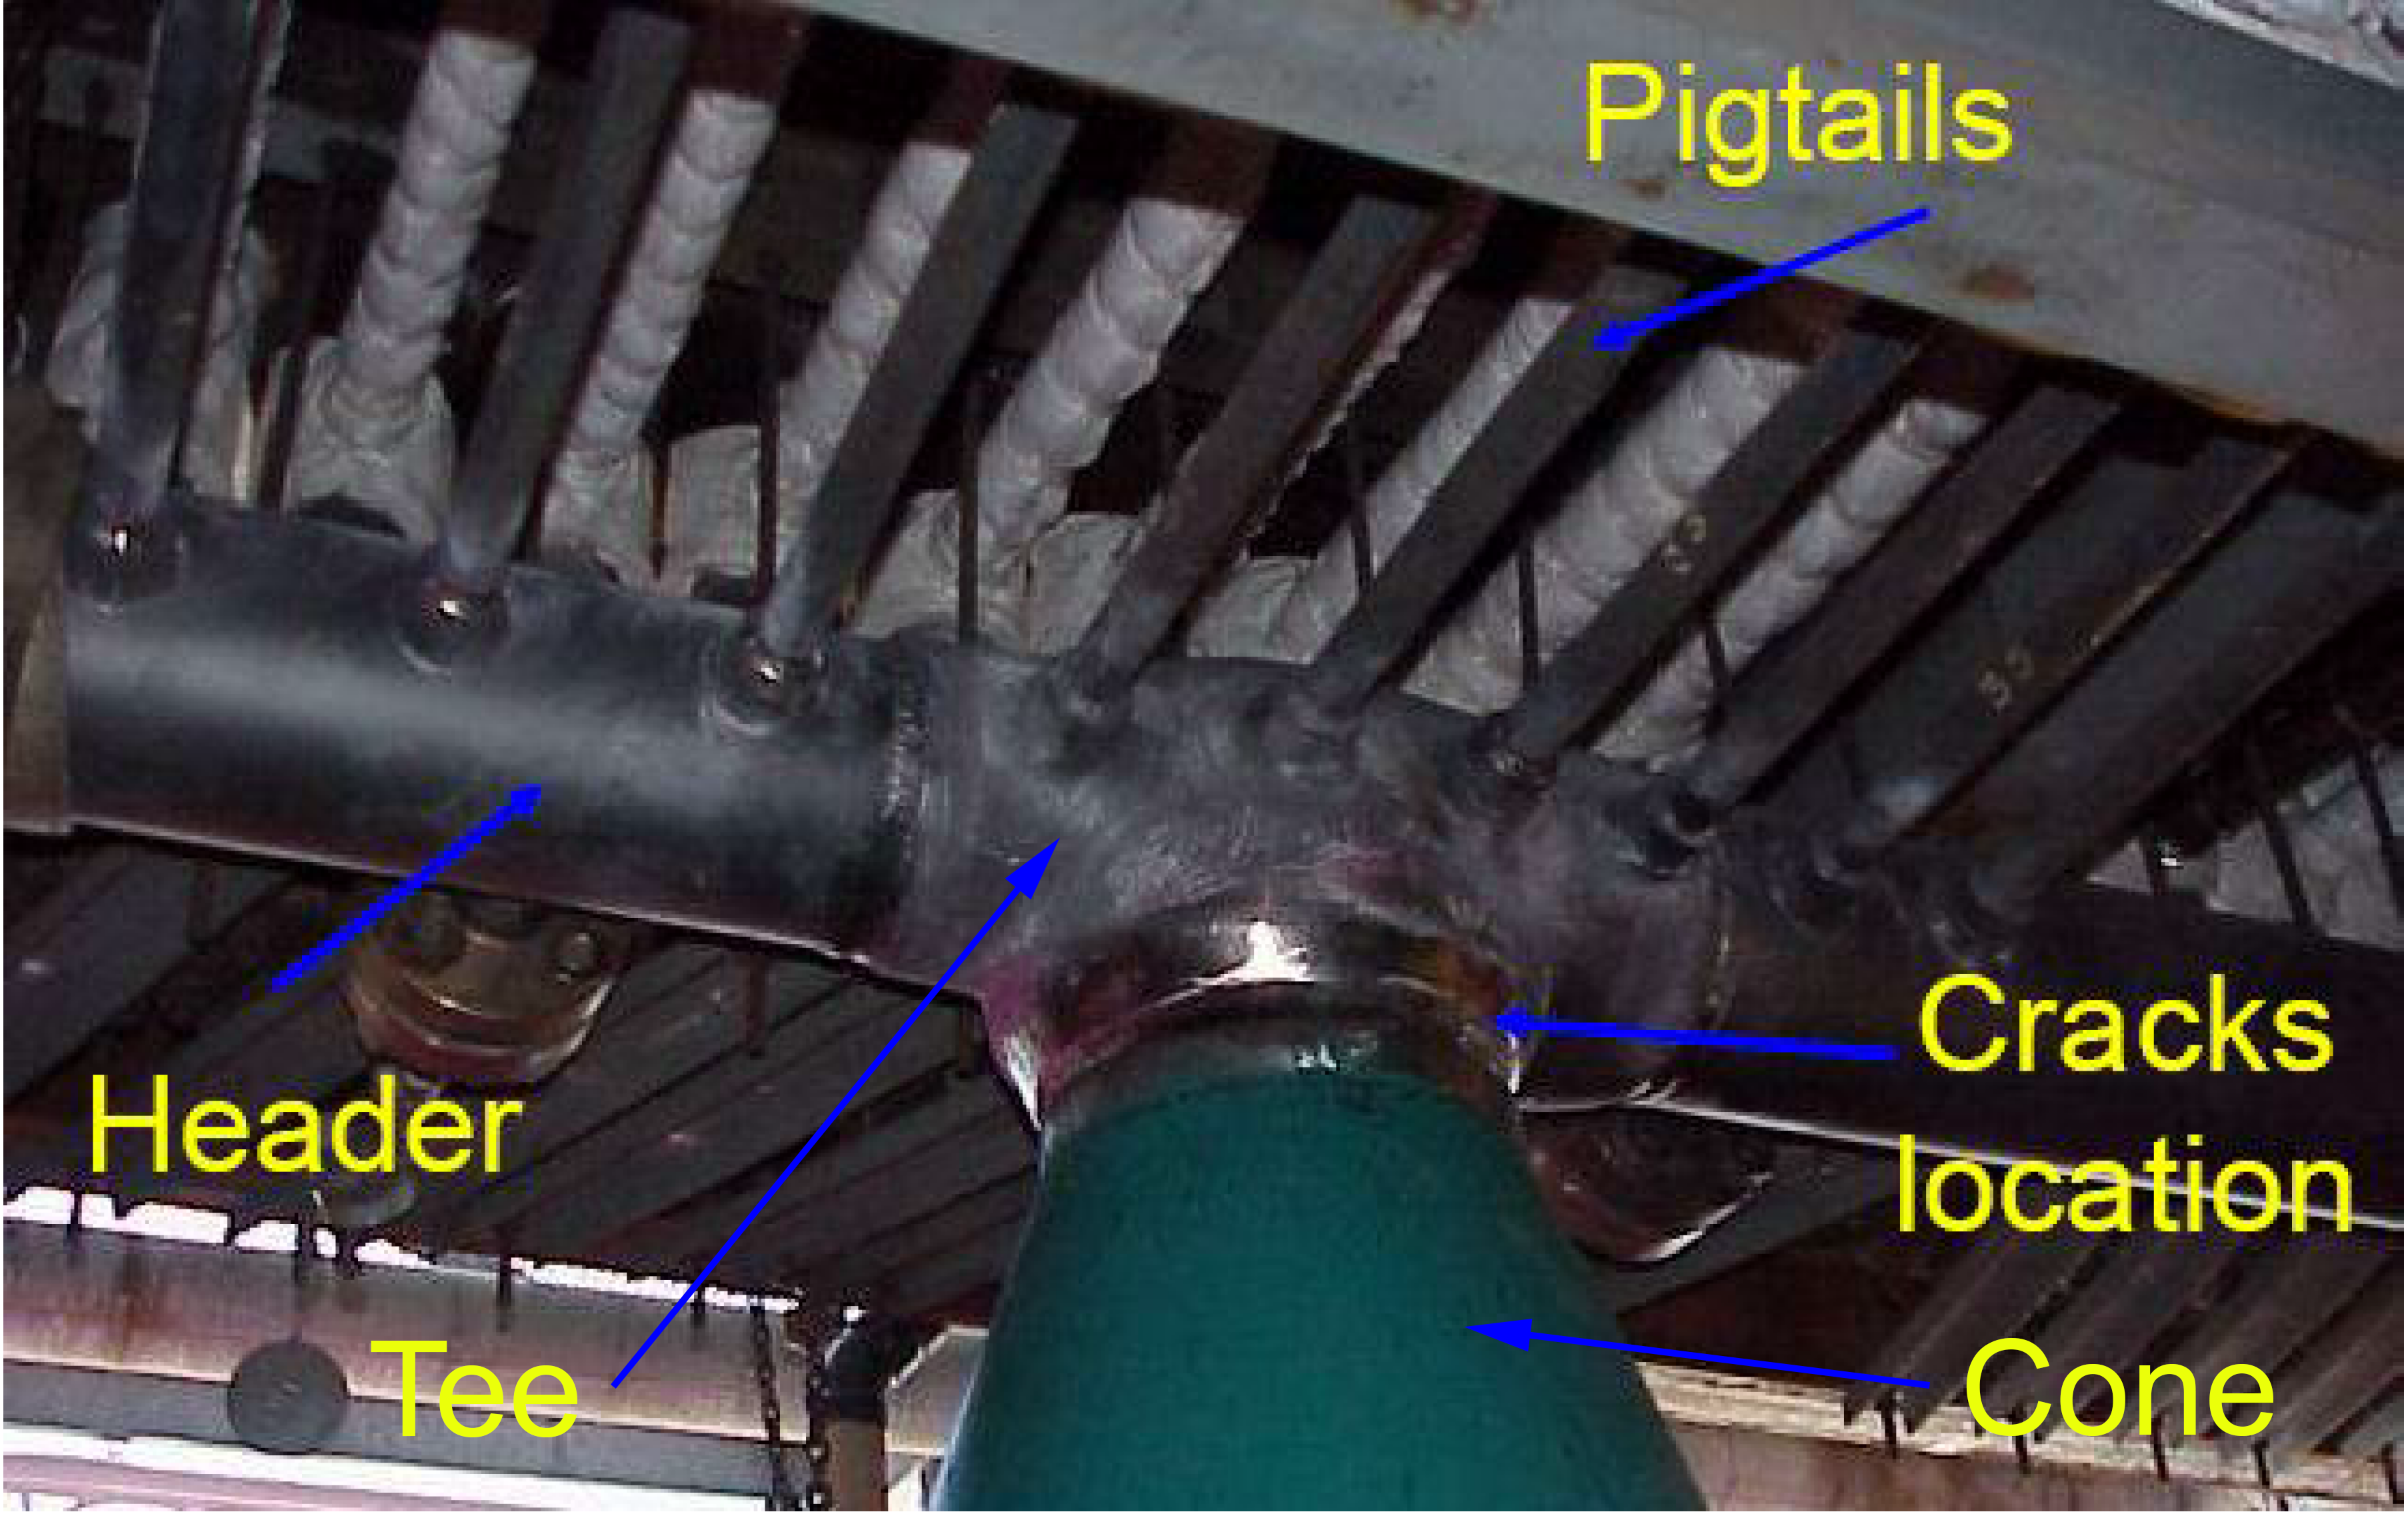
\includegraphics{figures/reformer-tee-cone}
\caption{Photograph of the outlet side of a reformer furnace, showing the outlet pigtails from the reformer catalyst tubes and the outlet header, tee, and cone which connect to the refractory-lined transfer system.  From \citet{penso_repair_2006}.}
\label{fig:reformer-tee-cone}
\end{figure}

Because high exit temperatures maximize the yield of hydrogen from the reformer \cite{haussinger_hydrogen_2000}, typical temperatures are in the range of 700--900C on the outlet side of the reformer furnace. Thus, the reformer tubes and outlet manifold require materials possessing excellent creep performance in addition to resistance to carburization and oxidation. The traditional choice for reformer tubes was centrifugally cast HK-40 (20Cr-25Ni) alloy \cite{rostrup-nielsen_catalytic_1984}, although this has been supplanted by newer alloys such as the HP-Modified alloys (25Cr-35Ni) due to higher creep strength \cite{schillmoller_hp-modified_1992}. For outlet manifold components, Alloy 800, HU-40 (19Cr-39Ni), and HK-40 have been used previously \cite{shibasaki_experience_1993}. The HU-40 and HK-40 alloys were implemented because they offered higher creep strength than Alloy 800, but they were discovered to have problems either with excessive thermal gradients (for HU-40), which was the same problem as originally experienced with Alloy 800, or with unacceptable loss of ductility after long-term service exposure (HK-40) \cite{shibasaki_experience_1993,collins_effect_1980}. To increase the ductilty after service exposure while maintaining high creep strength, a cast steel with the nominal composition of 20Cr-32Ni-Nb was developed \cite{collins_effect_1980}. This alloy, which is specified as Grade CT15C in ASTM A351 \cite{astm_a351_2010}, has similar creep strength to HK-40 \cite{shibasaki_experience_1993} with improved ductility after service-exposure. 

Despite these improvements over traditional alloys, over the years industry has become aware \cite{api_942_2014} that the 20Cr-32Ni-Nb alloy exhibits significant issues when it is subjected to repair welding after service exposure. These issues manifest primarily as cracking occurring in the base metal \gls{haz}, for example as reported by \citet{hoffman_weld_1998}. The cracking occurrences are not alleviated by changes to welding procedures, such as utilizing a more ductile filler metal, but rather are only prevented by high-temperature solution annealing (>2000\textdegree{}F) of the service-exposed material prior to welding. Thus the cracking issues are directly related to the microstructural changes which occur under service conditions (700--900C). The objective of the current work is to evaluate the weldability of service-exposed 20Cr-32Ni-Nb material, utilizing a well-established test method for characterizing the weldability of steels (the Gleeble hot ductility test), and to relate the hot ductility results to observed microstructural characteristics.


% Due to high exit temperatures in the range of 700--900C on the outlet side of the reformer furnace, the reformer tubes and outlet manifold require materials possessing excellent creep performance. 


% Because the efficiency of the reforming reactions are linked to the exit temperature, materials with excellent creep performance are necessary for both the reformer tubes and outlet manifold to enable high operating temperatures to ensure high yield.


% Because the efficiency of the reforming reactions are dependent upon maintaining a high exit temperature, materials with excellent creep performance are necessary for both the reformer tubes and outlet manifold to enable high operating temperatures to ensure high yield.


% how does tube creep properties influence tube design?


% Because the reaction in 1 is endothermic while 2 and 3 are exothermic, the overall heat balance is negative under most process conditions and external heat must be supplied. Thus, steam reforming occurs in a reformer furnace having numerous reformer tubes which contain the catalyst material and through which the reactants are passed. 



    %!TEX root = ..\ms-thesis.tex
\chapter{Literature Review} \label{ch:literature-review}

\section{Weldability Evaluation} \label{sec:weldability-evaluation}

\subsection{Characteristics of a Weldability Test}

\subsection{The Hot Ductility Test}

\subsubsection{Hot Ductility Evaluation Criteria}
In one of their early studies utilizing the Gleeble hot ductility test to evaluate a number of alloys, \citet{nippes_further_1957} classified the observed hot ductility responses of the various alloys into several categories, based on the shapes of the hot ductility curves: Classes H1 or H2 for the on-heating behavior and Classes C1, C2, or C3 for the on-cooling behavior. Schematic hot ductility curves illustrating the characteristics of each behavior class are shown in Figure~\ref{fig:nippes-criteria} and a brief text description for each is provided in Table~\ref{tab:nippes-classification}. Of the two on-heating behavior categories, Class H2 (Figure~\ref{fig:nippes-criteria}b) behavior was identified as being intrinsically sensitive to hot cracking. Class H1 behavior (Figure~\ref{fig:nippes-criteria}a) was not considered in and of itself indicative of a propensity for hot cracking and thus required the evaluation of on-cooling results to determine the material's susceptibility. With regard to the on-cooling categories, materials exhibiting Class C1 (Figure~\ref{fig:nippes-criteria}c) behavior were considered not sensitive to hot cracking. Class C2 and Class C3 behaviors (Figure~\ref{fig:nippes-criteria}d,e) were associated with a higher sensitivity to hot cracking, with Class C3 behavior indicating the greatest sensitivity. In particular, \citeauthor{nippes_further_1957} found that those materials in the study which were known to exhibit hot cracking, based on field experience, exhibited Class C3 behavior with on-cooling ductility of 40\% or less of the on-heating ductility. Thus, using the Nippes classification system, in most cases a material's on-cooling ductility response will be the major indicating factor regarding its hot cracking susceptibility. Materials exhibiting Class C3 on-cooling behavior with a low recovery of on-cooling ductility (0--40\% of on-heating ductility) can be identified as showing the greatest susceptibility to hot cracking.

% Nippes Criteria
%\bigskip
\begin{figure}[h]
\centering
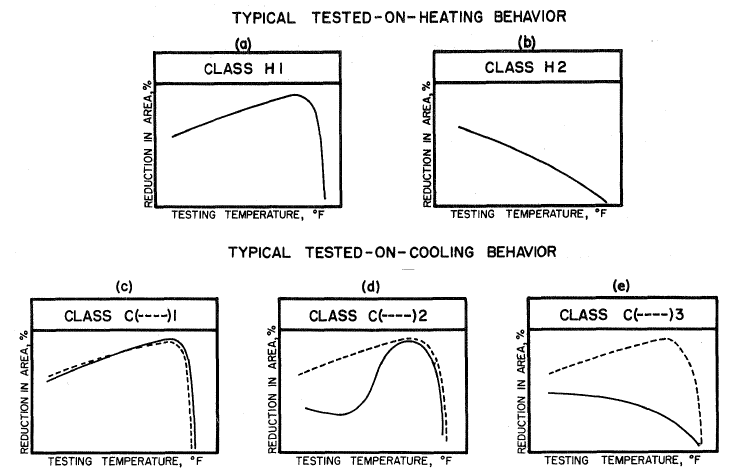
\includegraphics[width=6in]{figures/nippes-criteria.png}
\caption{Classification of Hot Ductility Behavior for On-heating and On-Cooling Tests; in (c), (d), and (e), the solid line is the on-cooling curve and the dashed line is the on-heating curve.  From \citet[Fig.~66]{nippes_further_1957}.}
\label{fig:nippes-criteria}
\end{figure}

\begin{table}[h]
\caption{Classification of on-heating and on-cooling hot ductility responses based on the work of \citet{nippes_further_1957}. Schematic curves for each behavior class are depicted in Figure~\ref{fig:nippes-criteria}.}
\begin{tabular}{ lp{4in} }
\toprule
\textbf{Classification} & \textbf{Description} \\
\midrule
On-Heating Class H1 & On-heating ductility generally increases as temperature increases, followed by a sudden loss of ductility over a relatively narrow range as the temperature increases further toward the melting point. (Figure~\ref{fig:nippes-criteria}a) \\
\addlinespace
On-Heating Class H2 & On-heating ductility shows a gradual decrease over a wide temperature range as the temperature increases toward the melting point. (Figure~\ref{fig:nippes-criteria}b) \\
& \\
On-Cooling Class C1 & On-cooling ductility is the essentially same as on-heating ductility at all test temperatures. (Figure~\ref{fig:nippes-criteria}c) \\
\addlinespace
On-Cooling Class C2 & On-cooling ductility is the same as on-heating ductility at test temperatures of 2100\textdegree{}F or above, but is significantly lower at test temperatures in the range of 1800--2000\textdegree{}F. (Figure~\ref{fig:nippes-criteria}d) \\
\addlinespace
On-Cooling Class C3 & On-cooling ductility is lower than on-heating ductility at all test temperatures; severity of ductility decrease may change with on-cooling test temperature or with the peak temperature utilized for the on-cooling thermal cycle. (Figure~\ref{fig:nippes-criteria}e) \\
\bottomrule
\end{tabular}
\label{tab:nippes-classification}
\end{table}


Further investigation of hot ductility test criteria was undertaken in a review by \citet{yeniscavich_correlation_1970}. One of the criteria reviewed, attributed to Nippes, was the \gls{drr}. According to this criteria, crack-resistant materials show a rapid recovery of on-cooling ductility after exposure to the \gls{haz} peak temperature, while the on-cooling ductility for crack-sensitive materials recovers slowly and remains low even at test temperatures well below the peak temperature. Schematic curves illustrating the \gls{drr} for crack-resistant and crack-sensitive materials are shown in Figure~\ref{fig:drr-schematic}. Numerically, the \gls{drr} is determined by taking the ratio of the on-cooling ductility to the on-heating ductility at a specified temperature, typically the rapid-ductility-decrease temperature on the on-heating curve (the point on the curve immediately prior to the sudden drop in ductility).

\begin{figure}
\centering
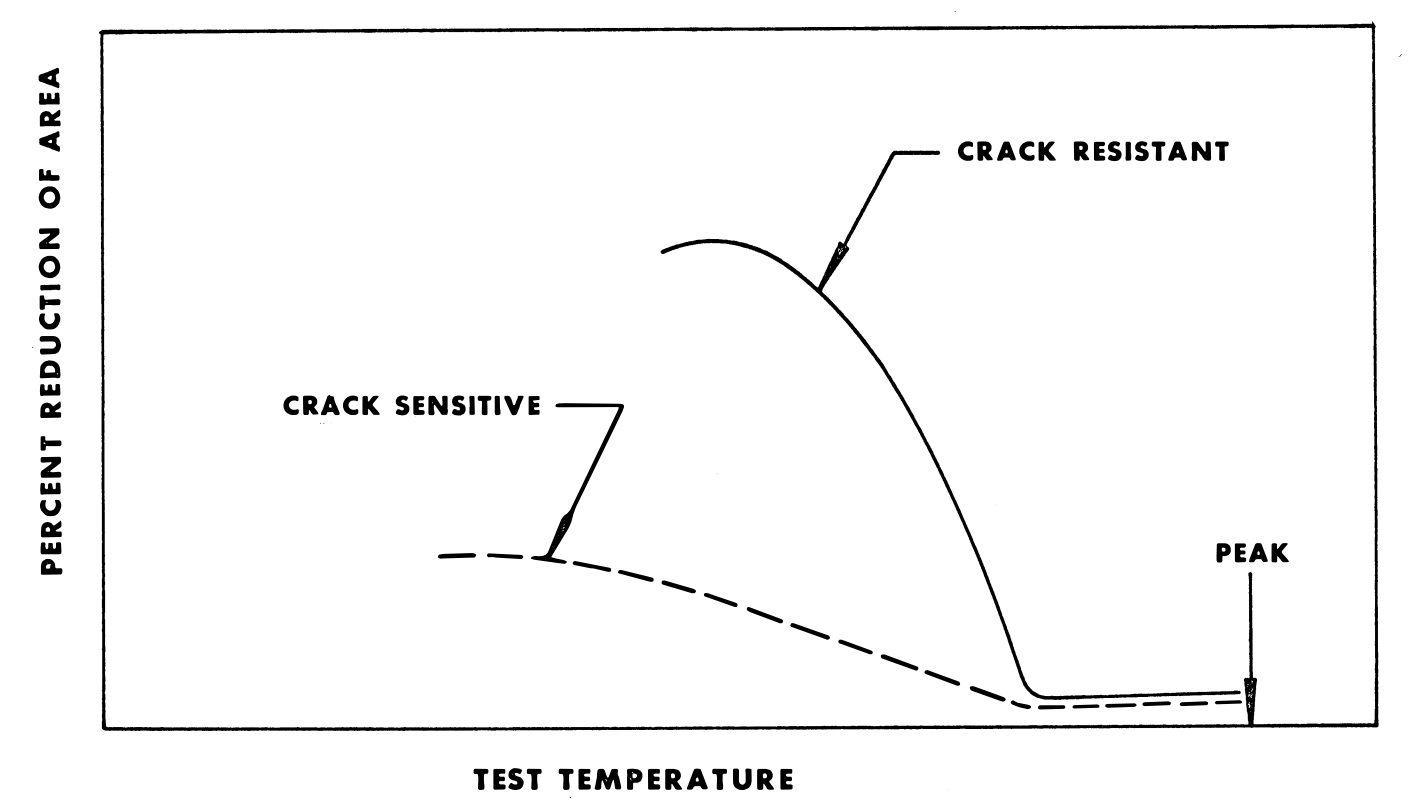
\includegraphics[width=6in]{figures/yeniscavich-drr.png}
\caption{Schematic curves illustrating the on-cooling \acrshort{drr} criteria for crack-resistant and crack-sensitive materials.  From \citet[Fig.~2]{yeniscavich_correlation_1970}}
\label{fig:drr-schematic}
\end{figure}

Yeniscavich also proposed the \gls{zdr} as an improved indicator of propensity for hot cracking. The \gls{zdr} phenomenon corresponds to a finite temperature increment below the ZDT in which the on-cooling ductility remains zero, i.e. the ductility does not immediately increase once the on-cooling test temperature is below the ZDT. The physical significance of the \gls{zdr} is related to the fact that the HAZ must possess sufficient ductility to withstand the thermal strains imposed during welding, otherwise cracking will occur. Since the magnitude of these strains is small over the length scale of an HAZ, the HAZ ductility must be on the order of zero for hot cracking to be of concern. Thus, alloys which show a large \gls{zdr} (zero ductility over a wide on-cooling temperature range) are considered more vulnerable to hot cracking than alloys which show a narrow \gls{zdr} (see Figure~\ref{fig:zdr-schematic}).

\begin{figure}
\centering
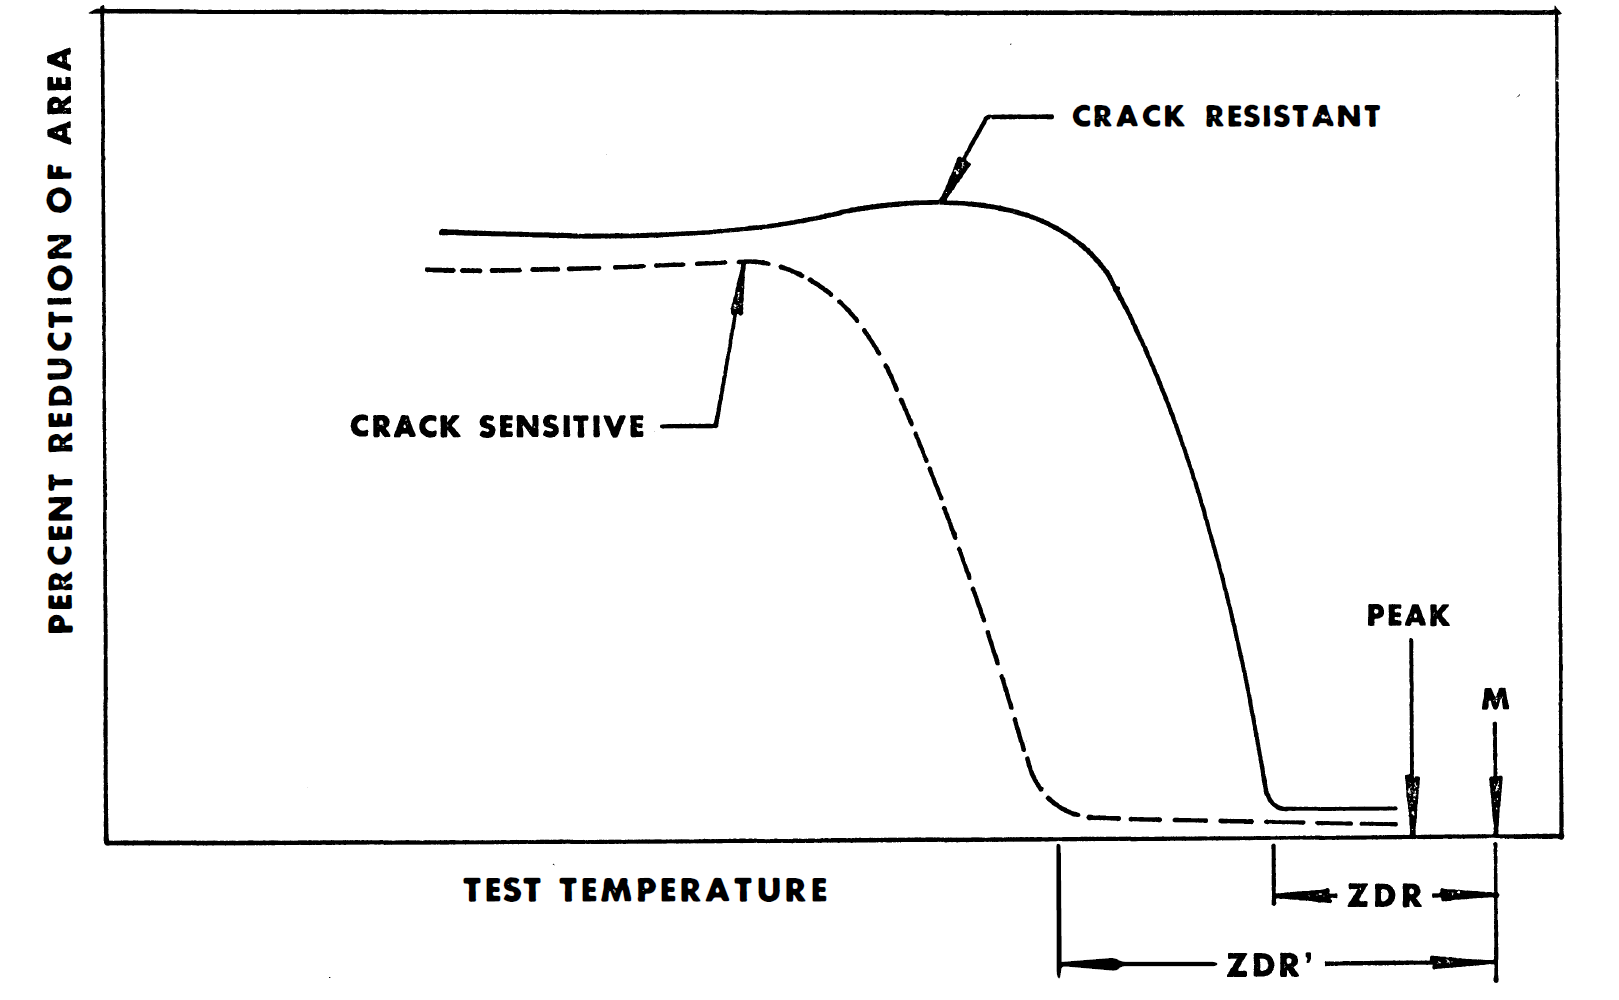
\includegraphics[width=6in]{figures/zdr-schematic.png}
\caption[Schematic of Hot Ductility Curves Illustrating Different On-Cooling Behaviors According to the Zero Ductility Range Criteria.]{Schematic of Hot Ductility Curves Illustrating Different On-Cooling Behaviors According to the Zero Ductility Range Criteria: Crack-Sensitive (\gls{zdr}') and Crack-Resistant (\gls{zdr}).  From \citet[Fig.~4]{yeniscavich_correlation_1970}}
\label{fig:zdr-schematic}
\end{figure}



    \chapter{Computational Fluid Dynamics}\label{ch:cfd}
    %!TEX root = ..\ms-thesis.tex
\chapter{Experimental Methods} \label{ch:experimental-methods}

\section{Hot Ductility Tests}
Standard hot ductility samples with dimensions of 114\,mm (4.5\,in) [length] by 6.35\,mm (0.25\,in) [diameter] were extracted from the Cone~1 and Cone~5 base metals adjacent to the respective cone-to-tee weld joints where cracking during repair welding had been observed.  A thermal cycle characteristic of \gls{smaw} with \SI[round-mode=places,round-precision=2]{2.75}{\kilo\joule\per\milli\meter} (\US{70}{\kilo\joule\per\inch}) energy input in 38\,mm (1.5\,in) stainless steel plate \cite{nippes_heat-affected_1955}, with an initial plate temperature of \SmartUnit{fahrenheit=80}, was utilized for the on-heating hot ductility tests.  This thermal cycle was determined based on the F(s,d) method \cite{nippes_cooling_1949} using data provided by Duffers Scientific \cite{duffers_haz_1989}. The peak temperature of the chosen thermal cycle was \SmartUnit{fahrenheit=2450}, equal to the estimated solidus temperature for the CT15C alloy based on data for Incoloy 800H (CT15C is considered a ``cast'' version of 800H) and which would roughly correspond to the maximum temperature experienced at the weld fusion line.

Once the on-heating hot ductility tests had been performed using the aforementioned thermal cycle and the \gls{zdt} had been determined, the thermal cycle was re-scaled so that the peak temperature coincided with the \gls{zdt}. The modified thermal cycle was subsequently used to perform the on-cooling hot ductility tests.  Both the on-heating and on-cooling tests were conducted according to the parameter guidelines recommended by a detailed study \cite{lundin_standardization_1990_experiment} undertaken to establish a standardized procedure for hot ductility testing.  The specific test parameters utilized in the current work are given in Table~\ref{tab:hot-ductility-parameters}.  For each test, the output of the control thermocouple was recorded, and the post-test cross-sectional area was determined and used to calculate the ductility in terms of percent reduction in area for each specimen.  The collected data were used to create plots of on-heating and on-cooling ductility (\% RA) as a function of test temperature.

\begin{table}[h]
\caption{Parameters and Conditions Used for Hot Ductility Testing, Based on Recommendations in \citet{lundin_standardization_1990_experiment}}
\begin{tabular}{ lp{4in} }
\toprule
\textbf{Parameter} & \textbf{Condition} \\
\midrule
Thermal Cycle & 38\,mm (1.5\,in) stainless steel plate, \gls{smaw} process, \SI[round-mode=places,round-precision=2]{2.75}{\kilo\joule\per\milli\meter} (\US{70}{\kilo\joule\per\inch}) energy input, \SmartUnit{fahrenheit=80} initial plate temperature \\
\addlinespace
Sample & 114\,mm (4.5\,in) length, 6.35\,mm (0.25\,in) diameter, 1/4-20 thread \\
\addlinespace
On-Cooling Peak Temp. & Zero Ductility Temperature determined from On-Heating Curve \\
\addlinespace
Crosshead Speed & \SI{50}{\milli\meter\per\second} (\US{2}{\inch\per\second}) \\
\addlinespace
Jaw Separation & 16\,mm (0.625 in) \\
\addlinespace
Control Thermocouple & 0.25\,mm (0.01\,in) diameter Chromel-Alumel; Percussion Welding / Separate attachment technique, \SI{1}{\milli\metre} wire spacing \\
\addlinespace
%Preload & \SIrange{3}{4}{\kilo\newton} \\
Test Atmosphere & Air \\
\bottomrule
\end{tabular}
\label{tab:hot-ductility-parameters}
\end{table}

\section{Microstructure Characterization}
Metallographic evaluations were conducted for the as-received Cone~1 and Cone~5 materials, utilizing remnants of the slices removed from the cones for machining of the hot ductility samples.  Metallography was also performed on selected hot ductility samples.  The hot ductility samples were sectioned longitudinally and mounted in castable epoxy and were subsequently ground and polished to a \SI[round-mode=places,round-precision=2]{0.05}{\micro\meter} finish.  The polished samples were electrolytically etched with an aqueous 10\% oxalic acid solution using a stainless steel cathode (\SI{50}{\milli\meter} (\US{2}{\inch}) spacing between the sample and cathode). For the as-received base metal samples, a potential of \SI{6}{\volt} for \SIrange[range-phrase=--]{3}{5}{\second} was used; for the hot ductility samples, it was found that a lower potential, \SI[round-mode=places,round-precision=1]{1.5}{\volt} for \SI{3}{\second}, was necessary to avoid excessive attack of certain phases near the fracture surfaces. \Gls{olm} examination of the etched samples was performed with a Nikon MA-200 inverted metallograph equipped with a 12 megapixel digital camera for obtaining micrographs. \Gls{sem} examination was conducted on selected samples using a LEO Gemini 1525 field emission \gls{sem} equipped with an Oxford Instruments PentaFet \gls{eds} system. Typically, a beam voltage of \SI{20}{\kilo\volt} was used for both \gls{se} and \gls{bse} imaging and for \gls{eds} analysis.
    %%%%%%%%%%%%%%%%%%%%%%%%%%%%%%%%%%%%%%%%%%%%%%%%%%%%%%%%%%%%%%%%%%%%%%%%%%%%%%%%%%%%%%%%%%%%%%%%%%%%%
    % BIBLIOGRAPHY
    %%%%%%%%%%%%%%%%%%%%%%%%%%%%%%%%%%%%%%%%%%%%%%%%%%%%%%%%%%%%%%%%%%%%%%%%%%%%%%%%%%%%%%%%%%%%%%%%%%%%%
    \makeBibliographyPage % make the bibliography title page - can be edited in ut-thesis-template.tex
    \bibliographystyle{apalike} % bibliography style - recommend using apalike-doi as it hyperlinks DOIs
    \bibliography{references/references-dissertation} % references.bib included in the references directory
    %%%%%%%%%%%%%%%%%%%%%%%%%%%%%%%%%%%%%%%%%%%%%%%%%%%%%%%%%%%%%%%%%%%%%%%%%%%%%%%%%%%%%%%%%%%%%%%%%%%%%
    % APPENDIX - OPTIONAL - COMMENT IF NOT NEEDED
    %%%%%%%%%%%%%%%%%%%%%%%%%%%%%%%%%%%%%%%%%%%%%%%%%%%%%%%%%%%%%%%%%%%%%%%%%%%%%%%%%%%%%%%%%%%%%%%%%%%%%
    \makeAppendixPage   % make the appendix title page - can be edited in ut-thesis-template.tex
    \appendix
    \chapter{Summary of Equations}
\section{Cartesian}
some equations here

\section{Cylindrical}
some equations also here
    %%%%%%%%%%%%%%%%%%%%%%%%%%%%%%%%%%%%%%%%%%%%%%%%%%%%%%%%%%%%%%%%%%%%%%%%%%%%%%%%%%%%%%%%%%%%%%%%%%%%%
    % A VITA IS REQUIRED
    %%%%%%%%%%%%%%%%%%%%%%%%%%%%%%%%%%%%%%%%%%%%%%%%%%%%%%%%%%%%%%%%%%%%%%%%%%%%%%%%%%%%%%%%%%%%%%%%%%%%%
    \addToTOC{Vita}
    \chapter*{Vita} \label{ch:vita}
John Bohling was born in Visalia, CA to his parents, Mark and Sandra Bohling. He is the oldest of four sons. After a cross-country move with his family, John attended Auburn High School in Auburn, AL, and graduated in 2005. After working for a year, he enrolled at the University of Tennessee, Knoxville in the fall of 2006. He graduated with a Bachelor of Science in Materials Science and Engineering in December 2010. During his undergraduate studies, his classes on metallurgy and welding sparked his interest in these areas, and the following year, he started his graduate studies at the University of Tennessee with Dr. Carl Lundin in the area of materials joining and welding metallurgy. John graduated with his Master of Science in Materials Science and Engineering, with a concentration in metallurgy, in August 2016. He is continuing his graduate work with Dr. Lundin at the University of Tennessee for a Ph.D. in Materials Science and Engineering.
\end{document}
